% Options for packages loaded elsewhere
\PassOptionsToPackage{unicode}{hyperref}
\PassOptionsToPackage{hyphens}{url}
%
\documentclass[
  ignorenonframetext,
]{beamer}
\usepackage{pgfpages}
\setbeamertemplate{caption}[numbered]
\setbeamertemplate{caption label separator}{: }
\setbeamercolor{caption name}{fg=normal text.fg}
\beamertemplatenavigationsymbolsempty
% Prevent slide breaks in the middle of a paragraph
\widowpenalties 1 10000
\raggedbottom
\setbeamertemplate{part page}{
  \centering
  \begin{beamercolorbox}[sep=16pt,center]{part title}
    \usebeamerfont{part title}\insertpart\par
  \end{beamercolorbox}
}
\setbeamertemplate{section page}{
  \centering
  \begin{beamercolorbox}[sep=12pt,center]{part title}
    \usebeamerfont{section title}\insertsection\par
  \end{beamercolorbox}
}
\setbeamertemplate{subsection page}{
  \centering
  \begin{beamercolorbox}[sep=8pt,center]{part title}
    \usebeamerfont{subsection title}\insertsubsection\par
  \end{beamercolorbox}
}
\AtBeginPart{
  \frame{\partpage}
}
\AtBeginSection{
  \ifbibliography
  \else
    \frame{\sectionpage}
  \fi
}
\AtBeginSubsection{
  \frame{\subsectionpage}
}
\usepackage{amsmath,amssymb}
\usepackage{iftex}
\ifPDFTeX
  \usepackage[T1]{fontenc}
  \usepackage[utf8]{inputenc}
  \usepackage{textcomp} % provide euro and other symbols
\else % if luatex or xetex
  \usepackage{unicode-math} % this also loads fontspec
  \defaultfontfeatures{Scale=MatchLowercase}
  \defaultfontfeatures[\rmfamily]{Ligatures=TeX,Scale=1}
\fi
\usepackage{lmodern}
\ifPDFTeX\else
  % xetex/luatex font selection
\fi
% Use upquote if available, for straight quotes in verbatim environments
\IfFileExists{upquote.sty}{\usepackage{upquote}}{}
\IfFileExists{microtype.sty}{% use microtype if available
  \usepackage[]{microtype}
  \UseMicrotypeSet[protrusion]{basicmath} % disable protrusion for tt fonts
}{}
\makeatletter
\@ifundefined{KOMAClassName}{% if non-KOMA class
  \IfFileExists{parskip.sty}{%
    \usepackage{parskip}
  }{% else
    \setlength{\parindent}{0pt}
    \setlength{\parskip}{6pt plus 2pt minus 1pt}}
}{% if KOMA class
  \KOMAoptions{parskip=half}}
\makeatother
\usepackage{xcolor}
\newif\ifbibliography
\usepackage{color}
\usepackage{fancyvrb}
\newcommand{\VerbBar}{|}
\newcommand{\VERB}{\Verb[commandchars=\\\{\}]}
\DefineVerbatimEnvironment{Highlighting}{Verbatim}{commandchars=\\\{\}}
% Add ',fontsize=\small' for more characters per line
\usepackage{framed}
\definecolor{shadecolor}{RGB}{248,248,248}
\newenvironment{Shaded}{\begin{snugshade}}{\end{snugshade}}
\newcommand{\AlertTok}[1]{\textcolor[rgb]{0.94,0.16,0.16}{#1}}
\newcommand{\AnnotationTok}[1]{\textcolor[rgb]{0.56,0.35,0.01}{\textbf{\textit{#1}}}}
\newcommand{\AttributeTok}[1]{\textcolor[rgb]{0.13,0.29,0.53}{#1}}
\newcommand{\BaseNTok}[1]{\textcolor[rgb]{0.00,0.00,0.81}{#1}}
\newcommand{\BuiltInTok}[1]{#1}
\newcommand{\CharTok}[1]{\textcolor[rgb]{0.31,0.60,0.02}{#1}}
\newcommand{\CommentTok}[1]{\textcolor[rgb]{0.56,0.35,0.01}{\textit{#1}}}
\newcommand{\CommentVarTok}[1]{\textcolor[rgb]{0.56,0.35,0.01}{\textbf{\textit{#1}}}}
\newcommand{\ConstantTok}[1]{\textcolor[rgb]{0.56,0.35,0.01}{#1}}
\newcommand{\ControlFlowTok}[1]{\textcolor[rgb]{0.13,0.29,0.53}{\textbf{#1}}}
\newcommand{\DataTypeTok}[1]{\textcolor[rgb]{0.13,0.29,0.53}{#1}}
\newcommand{\DecValTok}[1]{\textcolor[rgb]{0.00,0.00,0.81}{#1}}
\newcommand{\DocumentationTok}[1]{\textcolor[rgb]{0.56,0.35,0.01}{\textbf{\textit{#1}}}}
\newcommand{\ErrorTok}[1]{\textcolor[rgb]{0.64,0.00,0.00}{\textbf{#1}}}
\newcommand{\ExtensionTok}[1]{#1}
\newcommand{\FloatTok}[1]{\textcolor[rgb]{0.00,0.00,0.81}{#1}}
\newcommand{\FunctionTok}[1]{\textcolor[rgb]{0.13,0.29,0.53}{\textbf{#1}}}
\newcommand{\ImportTok}[1]{#1}
\newcommand{\InformationTok}[1]{\textcolor[rgb]{0.56,0.35,0.01}{\textbf{\textit{#1}}}}
\newcommand{\KeywordTok}[1]{\textcolor[rgb]{0.13,0.29,0.53}{\textbf{#1}}}
\newcommand{\NormalTok}[1]{#1}
\newcommand{\OperatorTok}[1]{\textcolor[rgb]{0.81,0.36,0.00}{\textbf{#1}}}
\newcommand{\OtherTok}[1]{\textcolor[rgb]{0.56,0.35,0.01}{#1}}
\newcommand{\PreprocessorTok}[1]{\textcolor[rgb]{0.56,0.35,0.01}{\textit{#1}}}
\newcommand{\RegionMarkerTok}[1]{#1}
\newcommand{\SpecialCharTok}[1]{\textcolor[rgb]{0.81,0.36,0.00}{\textbf{#1}}}
\newcommand{\SpecialStringTok}[1]{\textcolor[rgb]{0.31,0.60,0.02}{#1}}
\newcommand{\StringTok}[1]{\textcolor[rgb]{0.31,0.60,0.02}{#1}}
\newcommand{\VariableTok}[1]{\textcolor[rgb]{0.00,0.00,0.00}{#1}}
\newcommand{\VerbatimStringTok}[1]{\textcolor[rgb]{0.31,0.60,0.02}{#1}}
\newcommand{\WarningTok}[1]{\textcolor[rgb]{0.56,0.35,0.01}{\textbf{\textit{#1}}}}
\usepackage{longtable,booktabs,array}
\usepackage{calc} % for calculating minipage widths
\usepackage{caption}
% Make caption package work with longtable
\makeatletter
\def\fnum@table{\tablename~\thetable}
\makeatother
\usepackage{graphicx}
\makeatletter
\def\maxwidth{\ifdim\Gin@nat@width>\linewidth\linewidth\else\Gin@nat@width\fi}
\def\maxheight{\ifdim\Gin@nat@height>\textheight\textheight\else\Gin@nat@height\fi}
\makeatother
% Scale images if necessary, so that they will not overflow the page
% margins by default, and it is still possible to overwrite the defaults
% using explicit options in \includegraphics[width, height, ...]{}
\setkeys{Gin}{width=\maxwidth,height=\maxheight,keepaspectratio}
% Set default figure placement to htbp
\makeatletter
\def\fps@figure{htbp}
\makeatother
\setlength{\emergencystretch}{3em} % prevent overfull lines
\providecommand{\tightlist}{%
  \setlength{\itemsep}{0pt}\setlength{\parskip}{0pt}}
\setcounter{secnumdepth}{-\maxdimen} % remove section numbering
\ifLuaTeX
  \usepackage{selnolig}  % disable illegal ligatures
\fi
\IfFileExists{bookmark.sty}{\usepackage{bookmark}}{\usepackage{hyperref}}
\IfFileExists{xurl.sty}{\usepackage{xurl}}{} % add URL line breaks if available
\urlstyle{same}
\hypersetup{
  pdftitle={TMA4315 Generalized linear models H2018},
  pdfauthor={Mette Langaas, Department of Mathematical Sciences, NTNU - with contributions from Øyvind Bakke, Thea Bjørnland and Ingeborg Hem},
  hidelinks,
  pdfcreator={LaTeX via pandoc}}

\title{TMA4315 Generalized linear models H2018}
\subtitle{Module 3: BINARY REGRESSION}
\author{Mette Langaas, Department of Mathematical Sciences, NTNU - with
contributions from Øyvind Bakke, Thea Bjørnland and Ingeborg Hem}
\date{13.09 and 20.09 {[}PL{]}, 14.09 and 21.09 {[}IL{]}}

\begin{document}
\frame{\titlepage}

\begin{frame}
(Latest changes: 09.11: clarified one sentence on the devianc. 23.09:
score test moved to M4. 20.09: typos, and added solutions to Qs in
class. 18.09: typos and added sententence ILw2Problem3c. 16.09: edited
and added material for week 2, 13.09 moved material not lectured to
after the ILw1, and added one sentence to Problem 5 ILw1.)
\end{frame}

\begin{frame}{Overview}
\protect\hypertarget{overview}{}
\begin{block}{Learning material}
\protect\hypertarget{learning-material}{}
\begin{itemize}
\tightlist
\item
  Textbook: Fahrmeir et al (2013): Chapter 2.3, 5.1, B4.1-3
\item
  \href{https://www.math.ntnu.no/emner/TMA4315/2018h/TMA4315M3H20180913.pdf}{Classnotes
  13.09.2018}
\item
  \href{https://www.math.ntnu.no/emner/TMA4315/2018h/TMA4315M3H20180920.pdf}{Classnotes
  20.09.2018}
\end{itemize}
\end{block}
\end{frame}

\begin{frame}
\begin{block}{Topics}
\protect\hypertarget{topics}{}
\begin{block}{\protect\hyperlink{firstweek}{First week}}
\protect\hypertarget{first-week}{}
\begin{itemize}
\tightlist
\item
  aim of binary regression
\item
  how to model a binary response
\item
  three ingredients of a GLM model
\item
  the logit model: logistic regression
\item
  interpreting the logit model - with odds
\item
  grouped vs.~individual data
\item
  parameter estimation with maximum likelihood

  \begin{itemize}
  \tightlist
  \item
    likelihood, log-likelihood,
  \item
    score function
  \end{itemize}
\end{itemize}
\end{block}
\end{block}
\end{frame}

\begin{frame}[fragile]
\begin{block}{\protect\hyperlink{secondweek}{Second week}}
\protect\hypertarget{second-week}{}
\begin{itemize}
\tightlist
\item
  Parameter estimation

  \begin{itemize}
  \tightlist
  \item
    score function- and mean and covariance thereof,
  \item
    observed and expected information matrix
  \end{itemize}
\item
  comparison with the normal distribution - score function and Fisher
  information
\item
  exponential family and canonical link
\item
  iterative calculation of ML estimator (Newton-Raphson and Fisher
  scoring) - and in R with \texttt{optim}
\item
  asymptotic properties of ML estimators - how to use in inference?
\item
  statistical inference

  \begin{itemize}
  \tightlist
  \item
    confidence intervals
  \item
    hypothesis testing: Wald, and likelihood ratio
  \end{itemize}
\item
  deviance: definition, analysis of deviance, deviance residuals
\item
  model fit and model choice
\item
  overdispersion and estimating overdispersion parameter
\item
  sampling strategy: cohort, but also case-control data good for logit
  model
\end{itemize}
\end{block}
\end{frame}

\begin{frame}
\begin{block}{SECOND WEEK}
\protect\hypertarget{second-week-1}{}
Remember the \protect\hyperlink{beetle1}{beetle} and
\protect\hyperlink{infant1}{infant respitory disease} examples?

First, we look back at the \protect\hyperlink{binaryregassump}{model
requirements} for the binary regression - and the
\protect\hyperlink{loglik}{loglikelihood} and
\protect\hyperlink{score}{score function}.
\end{block}
\end{frame}

\begin{frame}{Likelihood and derivations thereof - continued}
\protect\hypertarget{likelihood-and-derivations-thereof---continued}{}
Individual data (not grouped):

Loglikelihood:
\[l(\boldsymbol{\beta})=\sum_{i=1}^n[y_i \ln \pi_i-y_i\ln(1-\pi_i)+\ln(1-\pi_i)]\]

Score function:
\[s(\boldsymbol{\beta})=\sum_{i=1}^n {\bf x}_i (y_i-\pi_i)\]
\end{frame}

\begin{frame}
\begin{block}{Properties of the score function}
\protect\hypertarget{properties-of-the-score-function}{}
Since the score function depends on \(Y_i=y_i\) we may regard the score
function as a random vector. We will now calculate the mean and
covariance matrix for the score function.
\end{block}
\end{frame}

\begin{frame}
\begin{block}{\(E(s(\boldsymbol{\beta}))\)}
\protect\hypertarget{esboldsymbolbeta}{}
The expected value of the score function is

\[
\begin{aligned}
E(s(\boldsymbol{\beta})) &= E(\sum_{i=1}^n(Y_i-\pi_i){\bf x}_i) \\
&= \sum_{i=1}^nE((Y_i-\pi_i){\bf x}_i) \\
&= \sum_{i=1}^n(E(Y_i)-\pi_i){\bf x}_i = 0 \\
\end{aligned}
\]

as \(E(Y_i) = \pi_i\).

We also see that
\(E(s_i(\boldsymbol{\beta})) = E((Y_i-\pi_i){\bf x}_i) = 0, \forall i\).
\end{block}
\end{frame}

\begin{frame}
\begin{block}{Fisher Information and Variances of Estimates}
\protect\hypertarget{fisher-information-and-variances-of-estimates}{}
The ``amount of information'' that the data carry about the parameters,
\(\boldsymbol{\beta}\), can be summarised by the curvature in the
likelihood surface

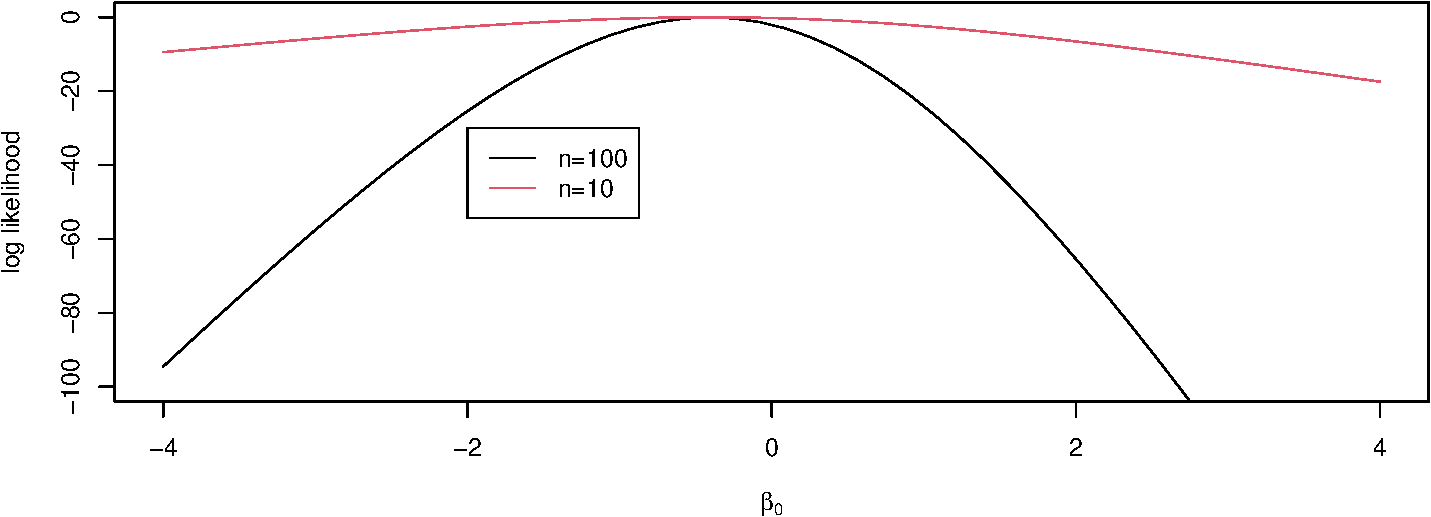
\includegraphics{Module03BinRegPresentationWeek2_files/figure-beamer/Curvature-1.pdf}
\end{block}
\end{frame}

\begin{frame}
\begin{block}{The expected Fisher information matrix
\(F(\boldsymbol{\beta})\)}
\protect\hypertarget{the-expected-fisher-information-matrix-fboldsymbolbeta}{}
The covariance of \(s(\boldsymbol{\beta})\) is called the expected
Fisher information matrix, \(F(\boldsymbol{\beta})\) and is given by

\[
\begin{aligned} 
F(\boldsymbol{\beta}) &= \text{Cov}(s(\boldsymbol{\beta})) = \sum_{i=1}^n \text{Cov}(s_i(\boldsymbol{\beta})) \\
&= \sum_{i=1}^n E\left[\Big(s_i(\boldsymbol{\beta}) - E(s_i(\boldsymbol{\beta}))\Big)\Big(s_i(\boldsymbol{\beta})-E(s_i(\boldsymbol{\beta}))\Big)^T\right] \\
&= \sum_{i=1}^n E(s_i(\boldsymbol{\beta})s_i(\boldsymbol{\beta})^T) = \sum_{i=1}^n F_i(\boldsymbol{\beta}) \end{aligned}
\]

assuming that the responses \(Y_i\) and \(Y_j\) are independent
\end{block}
\end{frame}

\begin{frame}
\begin{block}{\(F_i(\boldsymbol{\beta})\)}
\protect\hypertarget{f_iboldsymbolbeta}{}
Remember that \(s_i(\boldsymbol{\beta})=(Y_i-\pi_i){\bf x}_i\), then:

\[
\begin{aligned}
F_i(\boldsymbol{\beta}) &= E(s_i(\boldsymbol{\beta})s_i(\boldsymbol{\beta})^T) = E((Y_i-\pi_i){\bf x}_i(Y_i-\pi_i){\bf x}_i^T) \\
&= {\bf x}_i{\bf x}_i^T E((Y_i-\pi_i)^2)\\ 
&= {\bf x}_i{\bf x}_i^T \pi_i(1-\pi_i) 
\end{aligned}
\] where \(E((Y_i-\pi_i)^2)=\text{Var}(Y_i)=\pi_i(1-\pi_i)\) is the
variance of \(Y_i\). Thus

\[F(\boldsymbol{\beta}) = \sum_{i=1}^n {\bf x}_i{\bf x}_i^T \pi_i(1-\pi_i).\]
\end{block}
\end{frame}

\begin{frame}
\textbf{A useful relationship:} Under mild regularity conditions (so we
can change the order of \(\int\) and
\(\frac{\partial}{\partial \boldsymbol{\beta}}\)):

\[\text{Cov}(s(\boldsymbol{\beta}))=F(\boldsymbol{\beta}) = E\left( -\frac{\partial^2l(\boldsymbol{\beta})}{\partial\boldsymbol{\beta}\partial\boldsymbol{\beta}^T} \right) = E(-\text{Hessian matrix of }l)\]

which relates the expected to the observed Fisher information matrix.
\end{frame}

\begin{frame}
\begin{block}{Observed Fisher information matrix
\(H(\boldsymbol{\beta})\)}
\protect\hypertarget{observed-fisher-information-matrix-hboldsymbolbeta}{}
What is the observed Fisher information matrix? i.e.~don't take
expectations\ldots{}

\[H(\boldsymbol{\beta}) = -\frac{\partial^2l(\boldsymbol{\beta})}{\partial\boldsymbol{\beta}\partial\boldsymbol{\beta}^T} = -\frac{\partial s(\boldsymbol{\beta})}{\partial\boldsymbol{\beta}^T} = \frac{\partial}{\partial\boldsymbol{\beta}^T}\left[\sum_{i=1}^n (\pi_i-y_i){\bf x}_i \right] \]

because \(s(\boldsymbol{\beta}) = \sum_{i=1}^n (y_i-\pi_i){\bf x}_i\),
so \(-s(\boldsymbol{\beta}) = \sum_{i=1}^n (\pi_i-y_i){\bf x}_i\).

Note that \(\pi_i = \pi_i(\boldsymbol{\beta})\).
\end{block}
\end{frame}

\begin{frame}
\begin{block}{Calculating \(H(\boldsymbol{\beta})\)}
\protect\hypertarget{calculating-hboldsymbolbeta}{}
\[H(\boldsymbol{\beta}) = \sum_{i=1}^n \frac{\partial}{\partial\boldsymbol{\beta}^T}[{\bf x}_i\pi_i-{\bf x}_iy_i] = \sum_{i=1}^n \frac{\partial}{\partial\boldsymbol{\beta}^T}{\bf x}_i\pi_i = \sum_{i=1}^n {\bf x}_i \frac{\partial \pi_i}{\partial \eta_i} \frac{\partial \eta_i}{\partial \boldsymbol{\beta}^T} \]
\end{block}
\end{frame}

\begin{frame}
Use that

\[ \frac{\partial \eta_i}{\partial \boldsymbol{\beta}^T}=\frac{\partial {\bf x}_i^T\boldsymbol{\beta}}{\partial \boldsymbol{\beta}^T} = \left(\frac{\partial {\bf x}_i^T\boldsymbol{\beta}}{\partial \boldsymbol{\beta}}\right)^T = {\bf x}_i^T \]

and

\[
\begin{aligned}
\frac{\partial \pi_i}{\partial \eta_i} &=  \frac{\partial\left(\frac{\exp(\eta_i)}{1+\exp(\eta_i)}\right)}{\partial \eta_i}\\ &= \frac{(1+\exp(\eta_i))\exp(\eta_i) - \exp(\eta_i)\exp(\eta_i)}{(1+\exp(\eta_i))^2} \\
&= \frac{\exp(\eta_i)}{1+\exp(\eta_i)} \frac{1+\exp(\eta_i)-\exp(\eta_i)}{1+\exp(\eta_i)} \\
&=\pi_i (1-\pi_i).
\end{aligned}
\]
\end{frame}

\begin{frame}
And thus

\[
\begin{aligned}
H(\boldsymbol{\beta}) &=\sum_{i=1}^n {\bf x}_i \frac{\partial \pi_i}{\partial \eta_i} \frac{\partial \eta_i}{\partial \boldsymbol{\beta}^T} \\
&=\sum_{i=1}^n {\bf x}_i\pi_i(1-\pi_i) {\bf x}_i^T\\
&= \sum_{i=1}^n {\bf x}_i{\bf x}_i^T \pi_i(1-\pi_i).
\end{aligned}
\]

So the observed and the expected Fisher information matrix are equal.

This is not the case for the probit or complementary log-log models.
\end{frame}

\begin{frame}
\begin{block}{Overview of the results for individual and grouped data}
\protect\hypertarget{overview-of-the-results-for-individual-and-grouped-data}{}
\begin{itemize}
\tightlist
\item
  Individual data: \(i=1,\ldots, n\), and pairs \(({\bf x}_i,y_i)\).
\item
  Grouped data: \(j=1,\ldots, G\) with \(n_j\) observations for group
  \(j\), and \(Y_j=\sum Y_i\) for all \(i\) member of group \(j\). In
  total \(\sum_{j=1}^G n_j\) observations. For each pair
  \(({\bf x}_j, y_j)\), where \({\bf x}_j\) the covariate pattern for
  group \(j\).
\end{itemize}

NB: we keep that \(\eta_i=\ln (\frac{\pi_i}{1-\pi_i})\) - not changed
for grouped data (but now \(\mu_j=n_j\pi_j\)).
\end{block}
\end{frame}

\begin{frame}
\textbf{Log-likelihood:}

Individual:
\[l(\boldsymbol{\beta})=\sum_{i=1}^n[y_i \ln \pi_i-y_i\ln(1-\pi_i)+\ln(1-\pi_i)]\]
Grouped:
\[l(\boldsymbol{\beta})=\sum_{j=1}^G[y_j \ln \pi_j-y_j\ln(1-\pi_j)+n_j\ln(1-\pi_j)+ \ln {n_j \choose y_j}]\]
The last part is usually not include in calculations.
\end{frame}

\begin{frame}
\textbf{Score function:}

Individual: \[s(\boldsymbol{\beta})=\sum_{i=1}^n {\bf x}_i (y_i-\pi_i)\]

Grouped: \[s(\boldsymbol{\beta})=\sum_{j=1}^G {\bf x}_j (y_j-n_j\pi_j)\]
\end{frame}

\begin{frame}
\textbf{Expected Fisher information matrix:}

Individual:

\[F(\boldsymbol{\beta})=\sum_{i=1}^n {\bf x}_i {\bf x}_i^T\pi_i (1-\pi_i)\]

Grouped:

\[F(\boldsymbol{\beta})=\sum_{j=1}^G {\bf x}_j {\bf x}_j^T n_j \pi_j (1-\pi_j)\]

The observed Fisher information matrix equals the expected Fisher
information matrix - because the logit model is the \emph{canonical
link} for the binomial distribution.
\end{frame}

\begin{frame}
\begin{block}{Fitting the Models}
\protect\hypertarget{fitting-the-models}{}
There is no analytic solution, so we have to resort to numerics.
Luckily, these models behave well enough
\end{block}
\end{frame}

\begin{frame}
\begin{block}{Iterative gradient-based methods}
\protect\hypertarget{iterative-gradient-based-methods}{}
Use a first order multivariate Taylor approximation for
\(s(\hat{\boldsymbol{\beta}})\), around some chosen reference value
\(\boldsymbol{\beta}^{(0)}\):

\[
s(\hat{\boldsymbol{\beta}})\approx s(\boldsymbol{\beta}^{(0)})+\frac{\partial s(\boldsymbol{\beta})}{\partial \boldsymbol{\beta}}\big\rvert_{\boldsymbol{\beta}=\boldsymbol{\beta}^{(0)}} (\hat{\boldsymbol{\beta}}-\boldsymbol{\beta}^{(0)})
\]

Let
\(H(\boldsymbol{\beta}^{(0)})=-\frac{\partial s(\boldsymbol{\beta})}{\partial \boldsymbol{\beta}}\big\rvert_{\boldsymbol{\beta}=\boldsymbol{\beta}^{(0)}}\).
Setting \(s(\hat{\boldsymbol{\beta}})=0\) solving for
\(\hat{\boldsymbol{\beta}}\) gives

\[
\hat{\boldsymbol{\beta}}=\boldsymbol{\beta}^{(0)} + H(\boldsymbol{\beta}^{(0)})^{-1} s(\boldsymbol{\beta}^{(0)})
\] where \(H(\boldsymbol{\beta}^{(0)})^{-1}\) is the matrix inverse of
\(H(\boldsymbol{\beta}^{(0)})\).
\end{block}
\end{frame}

\begin{frame}
\begin{block}{Enter nNewton and Raphson}
\protect\hypertarget{enter-nnewton-and-raphson}{}
If we start with some value \(\boldsymbol{\beta}^{(0)}\) and then find a
new value \(\boldsymbol{\beta}^{(1)}\) by applying this equation, and
then continue applying the equation until convergence we have the
\emph{Newton-Raphson} method:

\[\boldsymbol{\beta}^{(t+1)}=\boldsymbol{\beta}^{(t)} + H(\boldsymbol{\beta}^{(t)})^{-1} s(\boldsymbol{\beta}^{(t)})\]
\end{block}
\end{frame}

\begin{frame}
Replacing the observed Fisher information matrix \({\bf H}\) with the
expected Fisher information matrix \({\bf F}\) yields the
\emph{Fisher-scoring} method.

For the logit model these two methods are the same since the observed
and expected Fisher information matrix is the same for canonical link
functions (like the logit is for binary regression).

This algorithm is run until the relative difference in Euclidean
distance between two iterations ``(new-old)/old'' is smaller than some
chosen constant.
\end{frame}

\begin{frame}
\begin{block}{Requirements for convergence}
\protect\hypertarget{requirements-for-convergence}{}
For the Newton-Raphson algorithm we see that the observed Fisher
information matrix \(H\) needs to be invertible for all
\(\boldsymbol{\beta}\), alternatively for the Fisher scoring algorithm
the expected Fisher information matrix \(F\) needs to be invertible.
\end{block}
\end{frame}

\begin{frame}
\begin{block}{Proof of convergence}
\protect\hypertarget{proof-of-convergence}{}
In our logit model
\[F(\boldsymbol{\beta})=\sum_{j=1}^G {\bf x}_j {\bf x}_j^T n_j \pi_j (1-\pi_j)\]

Let \({\bf X}\) be the design matrix, where the rows are
\({\bf x}_j^T\). Then
\({\bf X}^T{\bf X}=\sum_{j=1}^G {\bf x}_j {\bf x}_j^T\).

If we require that the design matrix has full rank (\(G\)) then also
\({\bf X}^T{\bf X}\) will have full rank (it will also be positive
definite) and and in addition \(\pi_j(1-\pi_j)>0\) for all
\(\pi_j \in (0,1)\), so then \(F(\boldsymbol{\beta})\) will be positive
definite and all is good.
\end{block}
\end{frame}

\begin{frame}
\begin{block}{Why is \(F(\boldsymbol{\beta})\) positive definite if we
require that the design matrix has full rank?}
\protect\hypertarget{why-is-fboldsymbolbeta-positive-definite-if-we-require-that-the-design-matrix-has-full-rank}{}
Formally, let \({\bf X}\) be a \(n\times p\) matrix and \(\Lambda\) a
\(n\times n\) diagonal matrix where all the diagonal elements are
positive (like our \(\pi_j(1-\pi_j)\), yes, put them on the diagonal).
Let \({\bf X}\) have independent columnes (full rank)
\(\Leftrightarrow\) \({\bf X}^T\Lambda{\bf X}\) is positive definite.

\emph{Proof:} \(\Rightarrow\): Let \({\bf v}\) be a \(p\) dimensional
column vector. Assume
\(0={\bf v}^T {\bf X}^T \Lambda {\bf X} {\bf v}=(\Lambda^{1/2}{\bf X}{\bf v})^T(\Lambda^{1/2}{\bf X}{\bf v})=\sum_{i=1}^n w_i^2\)
where \({\bf W}=\Lambda^{1/2}{\bf X}{\bf v}\). Then, \(w\) must be 0,
that is \(\Lambda^{1/2}{\bf X}{\bf v}=0\) since multiplication with
\(\Lambda^{1/2}\) is to multiply each element in \({\bf X}{\bf v}\) with
a number different from 0. That is, we must have \({\bf v}={\bf 0}\)
since \({\bf X}\) has independent columns.

\(\Leftarrow\): Assume that \({\bf X}{\bf v}={\bf 0}\). Then
\({\bf v}^T {\bf X}^T \Lambda {\bf X} {\bf v}={\bf 0}\) so
\({\bf v}={\bf 0}\) since \({\bf X}^T\Lambda{\bf X}\) is positive
definite. This is, \({\bf X}\) has independent columns.

\emph{End of proof}
\end{block}
\end{frame}

\begin{frame}
\begin{block}{We need a full rank}
\protect\hypertarget{we-need-a-full-rank}{}
Therefore, for GLMs we will also - as for the multiple linear regression
model in Module 2 - assume that the design matrix has full rank!

We will see in Module 5 that this is the requirement needed for GLMs in
general.
\end{block}
\end{frame}

\begin{frame}
\begin{block}{Convergence}
\protect\hypertarget{convergence}{}
Convergence is still not guarnateed, especially for small samples.

According to our text book, Fahrmeir et al (2013), page 284, the
conditions for uniqueness and existence of ML estimators are very
complex, and the authors suggest that the GLM user instead checks for
convergence in practice by performing the iterations.

In practice, the logit model most often causes problems, when (for
grouped data) \(y_i=0\) or \(y_i=n_i\), because \(\hat{\pi}_i=0/1\), so
\(\hat{\eta}_i=\pm \infty\). Computers do not like infinity
\end{block}
\end{frame}

\begin{frame}
stopped here
\end{frame}

\begin{frame}{Asymptotic properties of ML estimates}
\protect\hypertarget{asymptotic-properties-of-ml-estimates}{}
\begin{block}{Results}
\protect\hypertarget{results}{}
We need some weak regularity conditions, including

\begin{itemize}
\tightlist
\item
  \(\boldsymbol{\beta}\) falls in the interior of the parameter space
  and
\item
  \(p\) is fixed that \(n\) increases
\end{itemize}

(Agresti (2015) page 125):
\end{block}
\end{frame}

\begin{frame}
\begin{block}{The Results}
\protect\hypertarget{the-results}{}
Let \(\hat{\boldsymbol{\beta}}\) be the maximum likelihood (ML) estimate
in the GLM model. As the total sample size increases,
\(n\rightarrow \infty\):

\begin{enumerate}
\tightlist
\item
  \(\hat{\boldsymbol{\beta}}\) exists
\item
  \(\hat{\boldsymbol{\beta}}\) is consistent (convergence in
  probability, yielding asymptotically unbiased estimator, variances
  goes towards 0)
\item
  \(\hat{\boldsymbol{\beta}} \approx N_p(\boldsymbol{\beta},F^{-1}(\hat{\boldsymbol{\beta}}))\)
\end{enumerate}

So asymptotically
\(\text{Cov}(\hat{\boldsymbol{\beta}})=F^{-1}(\hat{\boldsymbol{\beta}})\):
the inverse of the expected Fisher information matrix evaluated at the
ML estimate.
\end{block}
\end{frame}

\begin{frame}
The \emph{proof} (for the univariate case) is given in the course
TMA4295 Statistical Inference course, Casella and Berger
(2002):``Statistical inference'', page 472.

Here we will sketch the proof. The strategy:

\begin{itemize}
\tightlist
\item
  make a first order Taylor expansion of the score function around the
  true parameter,
\item
  use the fact that the maximum likelihood estimate is defined as the
  zero of the score function.
\end{itemize}
\end{frame}

\begin{frame}
\begin{block}{The sketch}
\protect\hypertarget{the-sketch}{}
Use \(\boldsymbol{\theta}\) as the parameter of interest

(there is the connection to \(\boldsymbol{\mu}\), then to
\(\boldsymbol{\eta}\) and finally to \(\boldsymbol{\beta}\))

We start with the multivariate version of the first order Taylor
expansion of the score around the true parameter value
\(\boldsymbol{\theta}\):

\[s({\boldsymbol{\theta}}) \approx s(\hat{\boldsymbol{\theta}}) + s'({\boldsymbol{\theta}})(\hat{\boldsymbol{\theta}}-{\boldsymbol{\theta}})\]
As \(s'({\boldsymbol{\theta}}) = {\bf H}({\boldsymbol{\theta}})\), and
\(s(\hat{\boldsymbol{\theta}})=0\),

\[s(\hat{\boldsymbol{\theta}})\approx s({\boldsymbol{\theta}})-{\bf H}({\boldsymbol{\theta}})(\hat{\boldsymbol{\theta}}-{\boldsymbol{\theta}}) = 0\]

\[s({\boldsymbol{\theta}})\approx {\bf H}({\boldsymbol{\theta}})(\hat{\boldsymbol{\theta}}-{\boldsymbol{\theta}})\]
And premultiplying with \({\bf H}^{-1}(\boldsymbol{\theta})\) gives
\[ (\hat{\boldsymbol{\theta}}-{\boldsymbol{\theta}})\approx {\bf H}^{-1}({\boldsymbol{\theta}})s({\boldsymbol{\theta}})\]
\end{block}
\end{frame}

\begin{frame}
Then, to use the central limit theorem we need some smart manipulations
with \(n\), so we start by multiplying with \(\sqrt{n}\) and split that
into \(n\) and \(\frac{1}{\sqrt{n}}\).

\[ \sqrt{n}(\hat{\boldsymbol{\theta}}-{\boldsymbol{\theta}})\approx \sqrt{n}{\bf H}^{-1}({\boldsymbol{\theta}})s({\boldsymbol{\theta}})=(\frac{1}{n}{\bf H}({\boldsymbol{\theta}}))^{-1}\frac{1}{\sqrt{n}}s({\boldsymbol{\theta}})\]

From the central limit theorem:

\begin{enumerate}
[1)]
\item
  \(\frac{1}{n}{\bf H}(\boldsymbol{\theta})\) goes to the expected value
  which is \({\bf F}(\boldsymbol{\theta})\) (in probability),
\item
  the part \(\frac{1}{\sqrt{n}}s({\boldsymbol{\theta}})\) asymptotically
  goes to a random variable \(W\) that follows a multivariate normal
  with
  \({\bf W} \sim N({\bf 0},\frac{1}{n}{\bf F}(\boldsymbol{\theta}))\):

  \begin{itemize}
  \tightlist
  \item
    mean
    \(\text{E}(\frac{1}{\sqrt{n}}s({\boldsymbol{\theta}}))={\bf 0}\) and
    the
  \item
    covariance matrix is
    \(\text{Cov}(\frac{1}{\sqrt{n}}s({\boldsymbol{\theta}}))=\frac{1}{n}{\bf F}(\boldsymbol{\theta})\)
  \end{itemize}
\end{enumerate}
\end{frame}

\begin{frame}
\[
\sqrt{n}(\hat{\boldsymbol{\theta}}-{\boldsymbol{\theta}}) \approx \bf{F}^{-1}(\boldsymbol{\theta}){\bf W}
\]

On the right side here we have a multivariate normal distributed random
variable \(\bf{F}^{-1}(\boldsymbol{\theta}){\bf W}\) with mean
\({\bf 0}\) and covariance matrix
\[\text{Cov}({\bf F}^{-1}(\boldsymbol{\theta}){\bf W})={\bf F}^{-1}(\boldsymbol{\theta})\frac{1}{n}{\bf F}(\boldsymbol{\theta}){\bf F}^{-1}(\boldsymbol{\theta})=\frac{1}{n}{\bf F}^{-1}(\boldsymbol{\theta})\]

This leads to the wanted result:

\[ \hat{\boldsymbol{\theta}}\approx N(\boldsymbol{\theta},{\bf F}^{-1}(\boldsymbol{\theta}))\]

Due to the Slutsky theorem (from TMA4295 Statistical inference) this
also holds when \({\bf F}^{-1}(\boldsymbol{\theta}))\) is replaced by
\({\bf F}^{-1}(\hat{\boldsymbol{\theta}}))\).
\end{frame}

\begin{frame}{Parameter estimation}
\protect\hypertarget{parameter-estimation}{}
Parameter estimation can be based on grouped data - so now we use
\(Y_j \sim \text{bin}(n_j,\pi_j)\) from 1 above, but keep 2 and 3
unchanged. The number of groups is \(G\) and the total number of
observations is \(\sum_{j=1}^G n_j\).

\begin{itemize}
\item
  Likelihood=joint distribution, exponential family.
  \[ f(y\mid \theta)=\exp \left( \frac{y \theta-b(\theta)}{\phi}\cdot w + c(y, \phi, w) \right) \]
  where we have that \(\theta=\ln(\frac{\pi}{1-\pi})\) for the binomial
  distribution, which means that our logit model is gives the canonical
  link (remember, good properties!).
\item
  Log-likelihood
  \[l(\boldsymbol{\beta})=\sum_{j=1}^G[y_j \ln \pi_j-y_j\ln(1-\pi_j)+n_j\ln(1-\pi_j)+ \ln {n_j \choose y_j}]\]
\end{itemize}
\end{frame}

\begin{frame}
\begin{itemize}
\item
  Score function=vector of partial derivatives of log-likelihood. Find
  ML by solving \(s(\hat{\boldsymbol{\beta})})=0\) - but no closed form
  solutions.
  \[s(\boldsymbol{\beta})=\sum_{j=1}^G {\bf x}_j (y_j-n_j\pi_j)\]
\item
  Expected Fisher information matrix
  \[F(\boldsymbol{\beta})=\sum_{j=1}^G {\bf x}_j {\bf x}_j^T n_j \pi_j (1-\pi_j)\]
\item
  \(\hat{\boldsymbol{\beta}}\) found iteratively using Newton-Raphson or
  Fisher scoring
  \[\boldsymbol{\beta}^{(t+1)}=\boldsymbol{\beta}^{(t)} + F(\boldsymbol{\beta}^{(t)})^{-1} s(\boldsymbol{\beta}^{(t)})\]
\item
  \(\hat{\boldsymbol{\beta}} \approx N_p(\boldsymbol{\beta},F^{-1}(\hat{\boldsymbol{\beta}}))\)
\end{itemize}
\end{frame}

\begin{frame}{Further statistical inference}
\protect\hypertarget{further-statistical-inference}{}
Our further statistical inference (confidence intervals and hypotheses
tests) are based on the asymptotic distribution of the parameter
estimates
\[\hat{\boldsymbol{\beta}} \approx N_p(\boldsymbol{\beta},F^{-1}(\hat{\boldsymbol{\beta}}))\]
where \(F^{-1}(\hat{\boldsymbol{\beta}}))\) is the inverse of the
expected Fisher information matrix inserted
\(\hat{\boldsymbol{\beta}}\).

For the logit model we found that
\[F(\boldsymbol{\beta})=\sum_{j=1}^G {\bf x}_j {\bf x}_j^T n_j \pi_j (1-\pi_j)\]
So we would need to do \(\pi_j=\frac{\exp(\eta-j)}{1+\exp(\eta_j)}\) and
\(\eta_j={\bf x}_j^T\boldsymbol{\beta}\) as ``usual'', and then replace
\(\boldsymbol{\beta}\) with \(\hat{\boldsymbol{\beta}}\).

The asymptotic distribution still holds when we replace
\(\boldsymbol{\beta}\) with \(\hat{\boldsymbol{\beta}}\) in \({\bf F}\).
\end{frame}

\begin{frame}
If we make a diagonal matrix \({\bf W}\) with \(n_j \pi_j (1-\pi_j)\) on
the diagonal, then we may write the matrix \(F(\boldsymbol{\beta})\) in
matrix notation. As before \({\bf X}\) is the \(G\times p\) design
matrix.

\[F(\boldsymbol{\beta})=\sum_{j=1}^G {\bf x}_j {\bf x}_j^T n_j \pi_j (1-\pi_j)={\bf X}^T {\bf W} {\bf X}.\]
which means that
\(\text{Cov}(\hat{\boldsymbol{\beta}})=({\bf X}^T {\bf W} {\bf X})^{-1}\)
for the binomial model (remember that \(\hat{\boldsymbol{\beta}}\) comes
in with \(\hat{\pi}_j\) in \({\bf W}\)).

\textbf{Q:} How is this compared to the normal case?

A: \(F(\boldsymbol{\beta})=\frac{1}{\sigma^2}{\bf X}^T{\bf X}\), and the
inverse
\(\text{Cov}(\hat{\boldsymbol{\beta}})=({\bf X}^T {\bf X})^{-1}\sigma^2\).
\end{frame}

\begin{frame}
Let \({\bf A}(\boldsymbol{\beta})=F^{-1}(\hat{\boldsymbol{\beta}})\),
and \(a_{kk}(\hat{\boldsymbol{\beta}})\) is diagonal element number
\(k\).

For one element of the parameter vector:
\[ Z_k=\frac{\hat{\boldsymbol{\beta}}_k-\boldsymbol{\beta}_k}{\sqrt{\hat{a}_{kk}({\boldsymbol{\beta}})}}\]
is asymptotically standard normal. We will use this now!
\end{frame}

\begin{frame}
\begin{block}{Confidence intervals}
\protect\hypertarget{confidence-intervals}{}
In addition to providing a parameter estimate for each element of our
parameter vector \(\boldsymbol{\beta}\) we should also report a
\((1-\alpha)100\)\% confidence interval (CI) for each element.

We focus on element \(k\) of \(\boldsymbol{\beta}\), called
\(\boldsymbol{\beta}_k\). It is known that asympotically

\[
Z_k=\frac{\hat{\boldsymbol{\beta}}_k-\boldsymbol{\beta}_k}{\sqrt{{a}_{kk}(\hat{\beta})}} \sim N(0,1)
\]

We use that to form confidence intervals.

Let \(z_{\alpha/2}\) be such that \(P(Z_k>z_{\alpha/2})=\alpha/2\).
\end{block}
\end{frame}

\begin{frame}
We then use \[ P(-z_{\alpha/2}\le Z_k \le z_{\alpha/2})=1-\alpha\]
insert \(Z_k\) and solve for \(\beta_k\) to get
\[ P(\hat{\beta}_k-z_{\alpha/2}\sqrt{a_{kk}(\hat{\beta})}
\le \beta_k \le \hat{\beta}_k-z_{\alpha/2}\sqrt{a_{kk}(\hat{\boldsymbol{\beta}})})=1-\alpha\]

A \((1-\alpha)\)\% CI for \(\beta_k\) is when we insert numerical values
for the upper and lower limits.

\textbf{Q:} We write \(a_{kk}(\hat{\boldsymbol{\beta}})\). Why not
\(a_{kk}(\hat{\beta}_{kk})\)?
\end{frame}

\begin{frame}[fragile]
\begin{block}{Example with the beetle data}
\protect\hypertarget{example-with-the-beetle-data}{}
Again, we study our beetle data - in the grouped version.

Here we calculate the upper and lower limits of the confidence interval
using the formula.

\begin{Shaded}
\begin{Highlighting}[]
\NormalTok{fitgrouped}\OtherTok{=}\FunctionTok{glm}\NormalTok{(}\FunctionTok{cbind}\NormalTok{(y, n}\SpecialCharTok{{-}}\NormalTok{y) }\SpecialCharTok{\textasciitilde{}}\NormalTok{ ldose, }\AttributeTok{family =} \StringTok{"binomial"}\NormalTok{, }\AttributeTok{data =}\NormalTok{ investr}\SpecialCharTok{::}\NormalTok{beetle) }
\NormalTok{coeff}\OtherTok{=}\NormalTok{fitgrouped}\SpecialCharTok{$}\NormalTok{coefficients}
\NormalTok{sds}\OtherTok{=}\FunctionTok{sqrt}\NormalTok{(}\FunctionTok{diag}\NormalTok{(}\FunctionTok{summary}\NormalTok{(fitgrouped)}\SpecialCharTok{$}\NormalTok{cov.scaled))}
\NormalTok{alpha}\OtherTok{=}\FloatTok{0.05}
\NormalTok{lower}\OtherTok{=}\NormalTok{coeff}\SpecialCharTok{{-}}\FunctionTok{qnorm}\NormalTok{(}\DecValTok{1}\SpecialCharTok{{-}}\NormalTok{alpha}\SpecialCharTok{/}\DecValTok{2}\NormalTok{)}\SpecialCharTok{*}\NormalTok{sds}
\NormalTok{upper}\OtherTok{=}\NormalTok{coeff}\SpecialCharTok{+}\FunctionTok{qnorm}\NormalTok{(}\DecValTok{1}\SpecialCharTok{{-}}\NormalTok{alpha}\SpecialCharTok{/}\DecValTok{2}\NormalTok{)}\SpecialCharTok{*}\NormalTok{sds}
\FunctionTok{cbind}\NormalTok{(lower,upper)}
\end{Highlighting}
\end{Shaded}

\begin{verbatim}
##                 lower     upper
## (Intercept) -70.87144 -50.56347
## ldose        28.56265  39.97800
\end{verbatim}

\textbf{Q:} Explain what is done in the \texttt{R}-print-out.
\end{block}
\end{frame}

\begin{frame}
\begin{block}{Hypothesis testing}
\protect\hypertarget{hypothesis-testing}{}
There are three methods that are mainly used for testing hypotheses in
GLMs: - Wald test, - likelihood ratio test and - score test.

We will look at the first two.
\end{block}
\end{frame}

\begin{frame}
First, look at linear hypotheses: We study a binary regression model
with \(p=k+1\) covariates, and refer to this as model A (the larger
model). As for the multiple linear model we then want to investigate the
null and alternative hypotheses of the following type(s):

\begin{eqnarray*}
 H_0: \beta_{j}&=&0 \text{ vs. } H_1:\beta_j\neq 0\\
 H_0: \beta_{1}&=&\beta_{2}=\beta_{3}=0 \text{ vs. } H_1:\text{ at least one of these }\neq 0\\
 H_0: \beta_{1}&=&\beta_{2}=\cdots=\beta_{k}=0 \text{ vs. } H_1:\text{ at least one of these }\neq 0\\
 \end{eqnarray*}
\end{frame}

\begin{frame}
We call the restricted model (when the null hypotesis is true) model B,
or the smaller model.

These null hypotheses and alternative hypotheses can all be rewritten as
a linear hypothesis
\[H_0: {\bf C}{\bf \boldsymbol{\beta}}={\bf d} \text{ vs. } {\bf C}{\bf \boldsymbol{\beta}}\neq {\bf d} \]
by specifying \({\bf C}\) to be a \(r \times p\) matrix and \({\bf d}\)
to be a column vector of length \(d\).
\end{frame}

\begin{frame}
\begin{block}{The Wald test}
\protect\hypertarget{the-wald-test}{}
The Wald test statistic is given as:

\[
w=({\bf C}\hat{{\bf \boldsymbol{\beta}}}-{\bf d})^{\text T}[{\bf C}F^{-1}(\hat{\boldsymbol{\beta}}){\bf C}^{\text T}]^{-1}({\bf C}\hat{{\bf \boldsymbol{\beta}}}-{\bf d})
\] and measures the distance between the estimate
\({\bf C}\hat{\boldsymbol{\beta}}\) and the value under then null
hypothesis \({\bf d}\), weighted by the asymptotic covariance matrix of
\({\bf C}\hat{\boldsymbol{\beta}}\).

Remember:
\(\text{Cov}({\bf C}\hat{\boldsymbol{\beta}})={\bf C}F^{-1}(\hat{\boldsymbol{\beta}}){\bf C}^{\text T}\).

Asymptotically, under the null hypothesis \(w \sim \chi_r^2\)
distribution with (where \(r\) is the number of hypotheses tested).

\(P\)-values are calculated in the upper tail of the
\(\chi^2\)-distribution.

Observe: to perform the test you only need to fit the larger model (and
not the smaller).
\end{block}
\end{frame}

\begin{frame}
For the special case that we only test one regression parameter, for
example \(\beta_k\):
\[ H_0: \beta_k=0 \text{ vs. } H_1: \beta_k\neq 0.\] Now
\({\bf C}\hat{\boldsymbol{\beta}}=\beta_k\) and
\({\bf C}[F(\hat{\boldsymbol{\beta}})]^{-1}{\bf C}^{\text T}={\bf C}{\bf A}(\boldsymbol{\beta}){\bf C}^{\text T}=a_{kk}(\boldsymbol{\beta})\),
and the Wald test becomes
\[ (\hat{\beta}_k-\beta_k)[a_{kk}(\hat{\boldsymbol{\beta}})]^{-1}(\hat{\beta}_k-\beta_k)=\left(\frac{\hat{\beta}_k-\beta_k}{\sqrt{a_{kk}(\hat{\boldsymbol{\beta}})}}\right)^2=Z_k^2\]
so, asymptotically the square of the standard normal, which we know
follows a \(\chi^2\)-distribution with 1 degree of freedom.
\end{frame}

\begin{frame}[fragile]
\textbf{Q}: Explain what you find in the columns named \texttt{z\ value}
and \texttt{Pr(\textgreater{}\textbar{}z\textbar{})} below, and which
hypothesis tests these are related to. Are the hypothesis tests
performed using the Wald test?

\begin{Shaded}
\begin{Highlighting}[]
\FunctionTok{library}\NormalTok{(investr)}
\NormalTok{fitgrouped}\OtherTok{=}\FunctionTok{glm}\NormalTok{(}\FunctionTok{cbind}\NormalTok{(y,n}\SpecialCharTok{{-}}\NormalTok{y) }\SpecialCharTok{\textasciitilde{}}\NormalTok{ ldose, }\AttributeTok{family=}\StringTok{"binomial"}\NormalTok{, }
               \AttributeTok{data =}\NormalTok{ investr}\SpecialCharTok{::}\NormalTok{beetle) }
\NormalTok{knitr}\SpecialCharTok{::}\FunctionTok{kable}\NormalTok{(}\FunctionTok{summary}\NormalTok{(fitgrouped)}\SpecialCharTok{$}\NormalTok{coefficients, }\AttributeTok{digits=}\DecValTok{2}\NormalTok{)}
\end{Highlighting}
\end{Shaded}

\begin{longtable}[]{@{}lrrrr@{}}
\toprule\noalign{}
& Estimate & Std. Error & z value &
Pr(\textgreater\textbar z\textbar) \\
\midrule\noalign{}
\endhead
(Intercept) & -60.72 & 5.18 & -11.72 & 0 \\
ldose & 34.27 & 2.91 & 11.77 & 0 \\
\bottomrule\noalign{}
\end{longtable}
\end{frame}

\begin{frame}
\begin{block}{The likelihood ratio test}
\protect\hypertarget{the-likelihood-ratio-test}{}
The likelihood ratio test (LRT), which compares the likelihood of two
models.

\begin{itemize}
\tightlist
\item
  First we maximize the likelihood for model A (the larger model) to get
  \(L(\hat{\boldsymbol{\beta}}_A)\) and \(\hat{\boldsymbol{\beta}}_A\).
\item
  Then we maximize the likelihood for model B (the smaller model) to get
  \(L(\hat{\boldsymbol{\beta}}_B)\) and \(\hat{\boldsymbol{\beta}}_B\).
\end{itemize}
\end{block}
\end{frame}

\begin{frame}
The likelihood of the larger model (A) will always be larger or equal to
the likelihood of the smaller mode (B). (Why?)

The likelihood ratio statistic is defined as
\[- 2\ln \lambda=-2(\ln L(\hat{\boldsymbol{\beta}}_B)-\ln L(\hat{\boldsymbol{\beta}}_A)) \]
(so, \(-2\) times small minus large).
\end{frame}

\begin{frame}
Under weak regularity conditions the test statistic is approximately
\(\chi^2\)-distributed with degrees of freedom equal the difference in
the number of parameters in the large and the small model. This is
general - and not related to the GLM! More in TMA4295 Statistical
Inference!

\(P\)-values are calculated in the upper tail of the
\(\chi^2\)-distribution.

Observe: to perform the test you need to fit both the small and the
large model.

Notice: asymptotically the Wald and likelihood ratio test statistics
have the same distribution, but the value of the test statistics might
be different. How different?
\end{frame}

\begin{frame}[fragile]
For the beetle data we compare model A=model with \texttt{ldose} as
covariate with model B=model with only intercept. We use the
loglikelihood-function that we made for the lecture session for week 2.

\begin{Shaded}
\begin{Highlighting}[]
\FunctionTok{library}\NormalTok{(investr)}
\NormalTok{fitgrouped}\OtherTok{=}\FunctionTok{glm}\NormalTok{(}\FunctionTok{cbind}\NormalTok{(y, n}\SpecialCharTok{{-}}\NormalTok{y) }\SpecialCharTok{\textasciitilde{}}\NormalTok{ ldose, }\AttributeTok{family =} \StringTok{"binomial"}\NormalTok{, }\AttributeTok{data =}\NormalTok{ investr}\SpecialCharTok{::}\NormalTok{beetle) }
\NormalTok{fitnull}\OtherTok{=}\FunctionTok{glm}\NormalTok{(}\FunctionTok{cbind}\NormalTok{(y, n}\SpecialCharTok{{-}}\NormalTok{y) }\SpecialCharTok{\textasciitilde{}} \DecValTok{1}\NormalTok{, }\AttributeTok{family =} \StringTok{"binomial"}\NormalTok{, }\AttributeTok{data =}\NormalTok{ investr}\SpecialCharTok{::}\NormalTok{beetle) }

\NormalTok{loglik }\OtherTok{\textless{}{-}} \ControlFlowTok{function}\NormalTok{(par, args)\{}
\NormalTok{  y }\OtherTok{\textless{}{-}}\NormalTok{ args}\SpecialCharTok{$}\NormalTok{y; x }\OtherTok{\textless{}{-}}\NormalTok{ args}\SpecialCharTok{$}\NormalTok{x; n }\OtherTok{\textless{}{-}}\NormalTok{ args}\SpecialCharTok{$}\NormalTok{n}
\NormalTok{  res }\OtherTok{\textless{}{-}} \FunctionTok{sum}\NormalTok{(y}\SpecialCharTok{*}\NormalTok{x}\SpecialCharTok{\%*\%}\NormalTok{par }\SpecialCharTok{{-}}\NormalTok{ n}\SpecialCharTok{*}\FunctionTok{log}\NormalTok{(}\DecValTok{1} \SpecialCharTok{+} \FunctionTok{exp}\NormalTok{(x}\SpecialCharTok{\%*\%}\NormalTok{par)))}
  \FunctionTok{return}\NormalTok{(res)}
\NormalTok{\}}
\end{Highlighting}
\end{Shaded}
\end{frame}

\begin{frame}[fragile]
\begin{Shaded}
\begin{Highlighting}[]
\CommentTok{\# call this with parameters estimated under model A=larger model}
\NormalTok{beetleargs }\OtherTok{=} \FunctionTok{list}\NormalTok{(}\AttributeTok{y =}\NormalTok{ investr}\SpecialCharTok{::}\NormalTok{beetle}\SpecialCharTok{$}\NormalTok{y, }
            \AttributeTok{x =} \FunctionTok{cbind}\NormalTok{(}\FunctionTok{rep}\NormalTok{(}\DecValTok{1}\NormalTok{, }\FunctionTok{nrow}\NormalTok{(investr}\SpecialCharTok{::}\NormalTok{beetle)), investr}\SpecialCharTok{::}\NormalTok{beetle}\SpecialCharTok{$}\NormalTok{ldose), }
            \AttributeTok{n =}\NormalTok{ investr}\SpecialCharTok{::}\NormalTok{ beetle}\SpecialCharTok{$}\NormalTok{n)}

\NormalTok{llA}\OtherTok{=}\FunctionTok{loglik}\NormalTok{(}\FunctionTok{matrix}\NormalTok{(fitgrouped}\SpecialCharTok{$}\NormalTok{coefficients,}\AttributeTok{ncol=}\DecValTok{1}\NormalTok{),}\AttributeTok{args=}\NormalTok{beetleargs)}

\CommentTok{\# then the smaller model, then we set the coeff for ldose to 0. B=smaller model}
\NormalTok{llB}\OtherTok{=}\FunctionTok{loglik}\NormalTok{(}\FunctionTok{matrix}\NormalTok{(}\FunctionTok{c}\NormalTok{(fitnull}\SpecialCharTok{$}\NormalTok{coefficients,}\DecValTok{0}\NormalTok{),}\AttributeTok{ncol=}\DecValTok{1}\NormalTok{),}\AttributeTok{args=}\NormalTok{beetleargs)}
\NormalTok{lrt}\OtherTok{=}\SpecialCharTok{{-}}\DecValTok{2}\SpecialCharTok{*}\NormalTok{(llB}\SpecialCharTok{{-}}\NormalTok{llA)}
\NormalTok{lrt}
\end{Highlighting}
\end{Shaded}

\begin{verbatim}
## [1] 272.9702
\end{verbatim}

\begin{Shaded}
\begin{Highlighting}[]
\FunctionTok{pchisq}\NormalTok{(lrt,}\AttributeTok{df=}\DecValTok{1}\NormalTok{, }\AttributeTok{lower.tail =} \ConstantTok{FALSE}\NormalTok{)}
\end{Highlighting}
\end{Shaded}

\begin{verbatim}
## [1] 2.556089e-61
\end{verbatim}
\end{frame}

\begin{frame}[fragile]
\begin{Shaded}
\begin{Highlighting}[]
\FunctionTok{anova}\NormalTok{(fitnull, fitgrouped, }\AttributeTok{test=}\StringTok{"LRT"}\NormalTok{)}
\end{Highlighting}
\end{Shaded}

\begin{verbatim}
## Analysis of Deviance Table
## 
## Model 1: cbind(y, n - y) ~ 1
## Model 2: cbind(y, n - y) ~ ldose
##   Resid. Df Resid. Dev Df Deviance  Pr(>Chi)    
## 1         7    284.202                          
## 2         6     11.232  1   272.97 < 2.2e-16 ***
## ---
## Signif. codes:  0 '***' 0.001 '**' 0.01 '*' 0.05 '.' 0.1 ' ' 1
\end{verbatim}

\textbf{Q and A:} Here the small model is the model with only intercept
and the large is the one with dose as covariate. This means that the
null hypothesis is that ``the small model is preferred'' and our
\(p\)-value is very small, so we reject the null hyptheses and stick
with the model with dose as covariate. Observe that the LRT can be
performed using \texttt{anova}.
\end{frame}

\begin{frame}{Deviance}
\protect\hypertarget{deviance}{}
The \emph{deviance} is used to assess model fit and also for model
choice, and is based on the likelihood ratio test statistic.

\textbf{Saturated model:} One parmeter per group: estimate \(\pi_j\) by
the observed frequency for the group: \(\tilde{\pi}_j=\frac{y_j}{n_j}\).
Then \(\tilde{\pi}\) is a \(G\)-dimensional column vector with the
elements \(\tilde{\pi}_j\).

This ``imaginary model'' is called the \emph{saturated} model.

\textbf{Candidate model:} The model that we are investigated can be
thought of as a \emph{candidate} model. Then we maximize the likelihood
to get \(\hat{\boldsymbol{\beta}}\) \& thus \(\hat{\pi}_j\). Then
\(\hat{\pi}\) is a \(G\)-dimensional column vector with the elements
\(\hat{\pi}_j\).
\end{frame}

\begin{frame}
The \emph{deviance} is defined as the likelihood ratio statistic, where
we put the saturated model in place of the larger model A and our
candidate model in place of the smaller model B:

\[
\begin{aligned}
D&=-2(\ln L(\text{candidate model})-\ln L(\text{saturated model})) \\
&=-2(l(\hat{\pi})-l(\tilde{\pi}))=
-2\sum_{j=1}^G(l_j(\hat{\pi}_j)-l_j(\tilde{\pi}_j))
\end{aligned}
\]

For our logit model this can be written as (after some maths): \[ 
D=2\sum_{j=1}^G [y_j\ln(\frac{y_j}{n_j\hat{\pi}_j})+(n_j-y_j)\ln(\frac{n_j-y_j}{n_j-n_j\hat{\pi}_j})]
\]

Verify this by yourself.
\end{frame}

\begin{frame}
If our model is good, it should not be too far from the saturated model,
and we measure this distance by the deviance.

If we want to investigate the null hypothesis that ``our model fits the
data well'' to the negation, it is useful to know that asymptotically
\(D\) is distributed as \(\chi^2\) with \(G-p\) degrees of freedom (same
reason as for the likelihood ratio test statistic).

This result depends on \(n_j\) being large, hard to say how large (at
least 5 is a rule of thumb).
\end{frame}

\begin{frame}[fragile]
The deviance is in \texttt{summary.glm} outputted as ``Residual
deviance'', which we read off as 11.2322311. Let's check for our beetle
example by computing the formula for \(D\) directly:

\begin{Shaded}
\begin{Highlighting}[]
\NormalTok{D}\OtherTok{=}\FunctionTok{deviance}\NormalTok{(fitgrouped)}
\NormalTok{D}
\end{Highlighting}
\end{Shaded}

\begin{verbatim}
## [1] 11.23223
\end{verbatim}

\begin{Shaded}
\begin{Highlighting}[]
\NormalTok{G}\OtherTok{=}\FunctionTok{dim}\NormalTok{(investr}\SpecialCharTok{::}\NormalTok{beetle)[}\DecValTok{1}\NormalTok{]}
\NormalTok{G}
\end{Highlighting}
\end{Shaded}

\begin{verbatim}
## [1] 8
\end{verbatim}

\begin{Shaded}
\begin{Highlighting}[]
\NormalTok{p}\OtherTok{=}\DecValTok{2}
\DecValTok{1}\SpecialCharTok{{-}}\FunctionTok{pchisq}\NormalTok{(D,G}\SpecialCharTok{{-}}\NormalTok{p)}
\end{Highlighting}
\end{Shaded}

\begin{verbatim}
## [1] 0.08145881
\end{verbatim}

So, do we have a good fit?
\end{frame}

\begin{frame}
The null hypothesis is that the candiate model is equally good as the
saturated model. We do not reject this hypothesis at level 0.05. This
means that we are satisfied with the candidate model.

In the summary from glm also the socalled \emph{NULL deviance} is given.
This is the deviance when the candicate model is the model with only
intercept term present. This deviance asymptotically distributed as
\(\chi^2\) with \(G-1\) degrees of freedom.
\end{frame}

\begin{frame}[fragile]
\footnotesize

\begin{Shaded}
\begin{Highlighting}[]
\FunctionTok{summary}\NormalTok{(fitgrouped)}
\end{Highlighting}
\end{Shaded}

\begin{verbatim}
## 
## Call:
## glm(formula = cbind(y, n - y) ~ ldose, family = "binomial", data = investr::beetle)
## 
## Coefficients:
##             Estimate Std. Error z value Pr(>|z|)    
## (Intercept)  -60.717      5.181  -11.72   <2e-16 ***
## ldose         34.270      2.912   11.77   <2e-16 ***
## ---
## Signif. codes:  0 '***' 0.001 '**' 0.01 '*' 0.05 '.' 0.1 ' ' 1
## 
## (Dispersion parameter for binomial family taken to be 1)
## 
##     Null deviance: 284.202  on 7  degrees of freedom
## Residual deviance:  11.232  on 6  degrees of freedom
## AIC: 41.43
## 
## Number of Fisher Scoring iterations: 4
\end{verbatim}

\normalsize

\textbf{Q}: where is the deviance(s) here and how do we use these?
\end{frame}

\begin{frame}
\begin{block}{Analysis of deviance}
\protect\hypertarget{analysis-of-deviance}{}
In MLR we have seen that we may produce a sequential analysis of
variance (Type I) by adding more and more terms to the model and
comparing the scaled decrease in SSE by the scaled SSE of a full model.

For the binary regression we may adapt a similar strategy, but with
using the scaled change in deviance instead of the SSE.

We use the infant respiratory disease data as an example
\end{block}
\end{frame}

\begin{frame}[fragile]
\footnotesize

\begin{Shaded}
\begin{Highlighting}[]
\FunctionTok{library}\NormalTok{(faraway)}
\NormalTok{fit}\OtherTok{=}\FunctionTok{glm}\NormalTok{(}\FunctionTok{cbind}\NormalTok{(disease, nondisease)}\SpecialCharTok{\textasciitilde{}}\NormalTok{sex}\SpecialCharTok{*}\NormalTok{food,}\AttributeTok{family=}\FunctionTok{binomial}\NormalTok{(}\AttributeTok{link=}\NormalTok{logit),}\AttributeTok{data=}\NormalTok{babyfood)}
\FunctionTok{summary}\NormalTok{(fit)}
\end{Highlighting}
\end{Shaded}

\begin{verbatim}
## 
## Call:
## glm(formula = cbind(disease, nondisease) ~ sex * food, family = binomial(link = logit), 
##     data = babyfood)
## 
## Coefficients:
##                    Estimate Std. Error z value Pr(>|z|)    
## (Intercept)        -1.59899    0.12495 -12.797  < 2e-16 ***
## sexGirl            -0.34692    0.19855  -1.747 0.080591 .  
## foodBreast         -0.65342    0.19780  -3.303 0.000955 ***
## foodSuppl          -0.30860    0.27578  -1.119 0.263145    
## sexGirl:foodBreast -0.03742    0.31225  -0.120 0.904603    
## sexGirl:foodSuppl   0.31757    0.41397   0.767 0.443012    
## ---
## Signif. codes:  0 '***' 0.001 '**' 0.01 '*' 0.05 '.' 0.1 ' ' 1
## 
## (Dispersion parameter for binomial family taken to be 1)
## 
##     Null deviance: 2.6375e+01  on 5  degrees of freedom
## Residual deviance: 4.2144e-13  on 0  degrees of freedom
## AIC: 43.518
## 
## Number of Fisher Scoring iterations: 3
\end{verbatim}

\begin{Shaded}
\begin{Highlighting}[]
\FunctionTok{anova}\NormalTok{(fit,}\AttributeTok{test=}\StringTok{"Chisq"}\NormalTok{)}
\end{Highlighting}
\end{Shaded}

\begin{verbatim}
## Analysis of Deviance Table
## 
## Model: binomial, link: logit
## 
## Response: cbind(disease, nondisease)
## 
## Terms added sequentially (first to last)
## 
## 
##          Df Deviance Resid. Df Resid. Dev  Pr(>Chi)    
## NULL                         5    26.3753              
## sex       1   5.4761         4    20.8992   0.01928 *  
## food      2  20.1772         2     0.7219 4.155e-05 ***
## sex:food  2   0.7219         0     0.0000   0.69701    
## ---
## Signif. codes:  0 '***' 0.001 '**' 0.01 '*' 0.05 '.' 0.1 ' ' 1
\end{verbatim}

\normalsize

\textbf{Q}: is it recommended (from the test) to add an interaction term
to the model? What does it mean that the Residual deviance is 0 for the
\texttt{sex*food} model?
\end{frame}

\begin{frame}
\begin{block}{Deviance residuals}
\protect\hypertarget{deviance-residuals}{}
The deviance residuals are given by a signed version of each element in
the sum for the deviance, that is
\[d_k=\text{sign}(y_k-n_k\hat{\pi}_k)\cdot \left\{ 
2[y_k\ln(\frac{y_k}{n_k\hat{\pi}_k})+(n_k-y_k)\ln(\frac{n_k-y_k}{n_k-n_k\hat{\pi}_k})]\right\}^{1/2}\]
where the term \(\text{sign}(y_k-n_k\hat{\pi}_k)\) makes negative
residuals possible.
\end{block}
\end{frame}

\begin{frame}{Model assessment and choice}
\protect\hypertarget{model-assessment-and-choice}{}
The fit of the model can be assessed based on goodness of fit statistics
(and related tests) and by residual plots. Model choice can be made from
analysis of deviance, or by comparing the AIC for different models.

\begin{block}{Deviance test for grouped data}
\protect\hypertarget{deviance-test-for-grouped-data}{}
We may use the deviance test presented before to test if the model under
study is preferred compared to the saturated model.
\end{block}
\end{frame}

\begin{frame}
\begin{block}{Pearson test and residuals}
\protect\hypertarget{pearson-test-and-residuals}{}
An alternative to the deviance test is the Pearson test. We will look in
more detail at this test in a Module 4. The Pearson test statistic can
be written as a function of the Pearson residuals, which for the
binomial regression is given as:
\[ r_{j}=\frac{y_j-n_j\hat{\pi}_j}{\sqrt{n_j \hat{\pi}_j(1-\hat{\pi}_j)}}\]
Remark: A standardized version scales the Pearson residuals with
\(\sqrt{1-h_{kk}}\) similar to the standardized residuals for the normal
model. Here \(h_{kk}\) is the diagonal element number \(k\) in the hat
matrix \({\bf H}={\bf X}({\bf X}^T{\bf X})^{-1}{\bf X}^T\).
\end{block}
\end{frame}

\begin{frame}
The Pearson \(\chi^2\)-goodness of fit statistic is given as
\[ X_P^2=\sum_{j=1}^G r_j^2=\sum_{j=1}^G  \frac{(y_j-n_j\hat{\pi}_j)^2}{n_j \hat{\pi}_j(1-\hat{\pi}_j)}\]
The Pearson \(\chi^2\) statistic is asymptotically equivalent to the
deviance statistic and thus is asymptotically \(\chi^2_{G-p}\).

The Pearson \(\chi^2\) statistic is not a good choice if any of the
groups have a low expected number of observations,
i.e.~\(n_j \hat{\pi}_j\) is small (below 1).
\end{frame}

\begin{frame}
\begin{block}{Model assessment with continuous covariates}
\protect\hypertarget{model-assessment-with-continuous-covariates}{}
If data have continuous covariates it is possible to form groups based
making intervals for continuous covariates. Alternatively grouping on
predicted probabilites can be done.

For continuous data the Hosmer Lemeshow test can be used - not on our
reading list.
\end{block}
\end{frame}

\begin{frame}
\begin{block}{Plotting residuals}
\protect\hypertarget{plotting-residuals}{}
Deviance and Pearson residuals can be used for checking the fit of the
model, by plotting the residuals against fitted values and covariates.

If \(n_j\) is small for the covariate patterns the residual plots may be
relatively uninformative.

Residual plots for the logistics regression - and for the GLM in general
- is highly debated, and we will not put much emphasis on residual plots
for this module.
\end{block}
\end{frame}

\begin{frame}
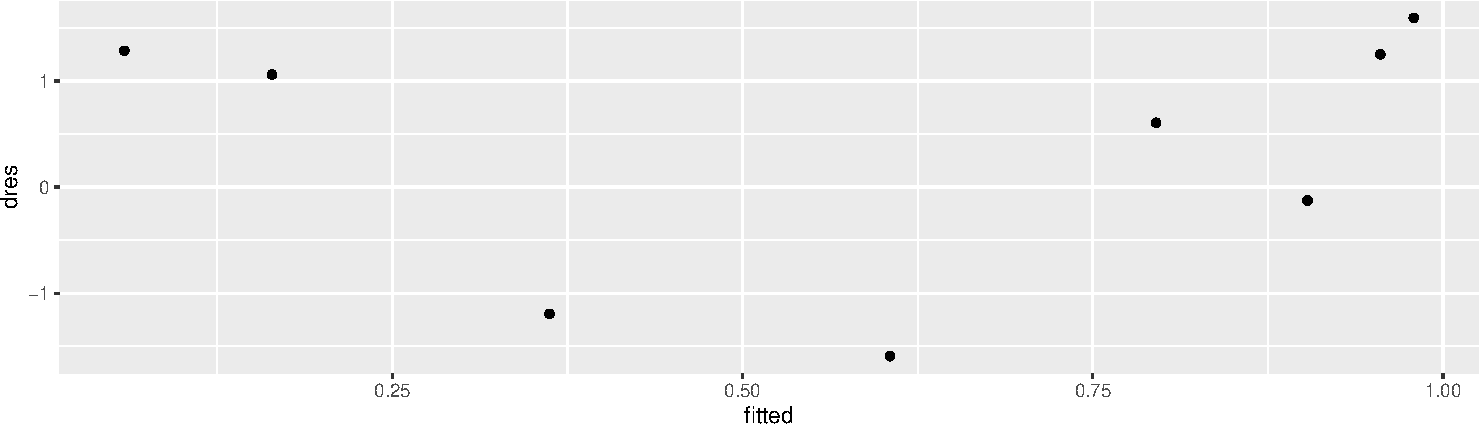
\includegraphics{Module03BinRegPresentationWeek2_files/figure-beamer/unnamed-chunk-10-1.pdf}
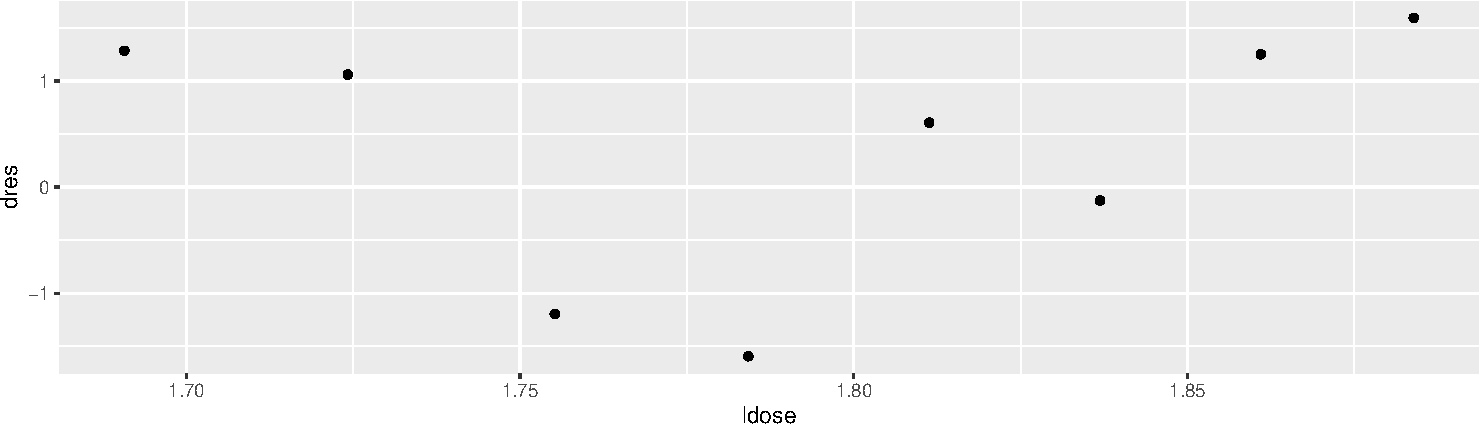
\includegraphics{Module03BinRegPresentationWeek2_files/figure-beamer/unnamed-chunk-10-2.pdf}
\end{frame}

\begin{frame}[fragile]
\begin{block}{Other plots}
\protect\hypertarget{other-plots}{}
A useful plot is to show observed and fitted proportions (grouped data)
plotted against the linear predictor or covariates.

\begin{Shaded}
\begin{Highlighting}[]
\FunctionTok{library}\NormalTok{(ggplot2)}
\NormalTok{df}\OtherTok{=}\FunctionTok{data.frame}\NormalTok{(}\StringTok{"fitted"}\OtherTok{=}\NormalTok{fitgrouped}\SpecialCharTok{$}\NormalTok{fitted.values,}\StringTok{"dres"}\OtherTok{=}\FunctionTok{residuals}\NormalTok{(fitgrouped,}\AttributeTok{type=}\StringTok{"deviance"}\NormalTok{),}\StringTok{"ldose"}\OtherTok{=}\NormalTok{investr}\SpecialCharTok{::}\NormalTok{beetle}\SpecialCharTok{$}\NormalTok{ldose,}\StringTok{"frac"}\OtherTok{=}\NormalTok{investr}\SpecialCharTok{::}\NormalTok{beetle}\SpecialCharTok{$}\NormalTok{y}\SpecialCharTok{/}\NormalTok{investr}\SpecialCharTok{::}\NormalTok{beetle}\SpecialCharTok{$}\NormalTok{n)}
\FunctionTok{ggplot}\NormalTok{(df,}\FunctionTok{aes}\NormalTok{(}\AttributeTok{x=}\NormalTok{ldose))}\SpecialCharTok{+}\FunctionTok{geom\_point}\NormalTok{(}\FunctionTok{aes}\NormalTok{(}\AttributeTok{y=}\NormalTok{frac,}\AttributeTok{colour=}\StringTok{"observed"}\NormalTok{))}\SpecialCharTok{+}\FunctionTok{geom\_point}\NormalTok{(}\FunctionTok{aes}\NormalTok{(}\AttributeTok{y=}\NormalTok{fitted,}\AttributeTok{colour=}\StringTok{"fitted"}\NormalTok{))}
\end{Highlighting}
\end{Shaded}

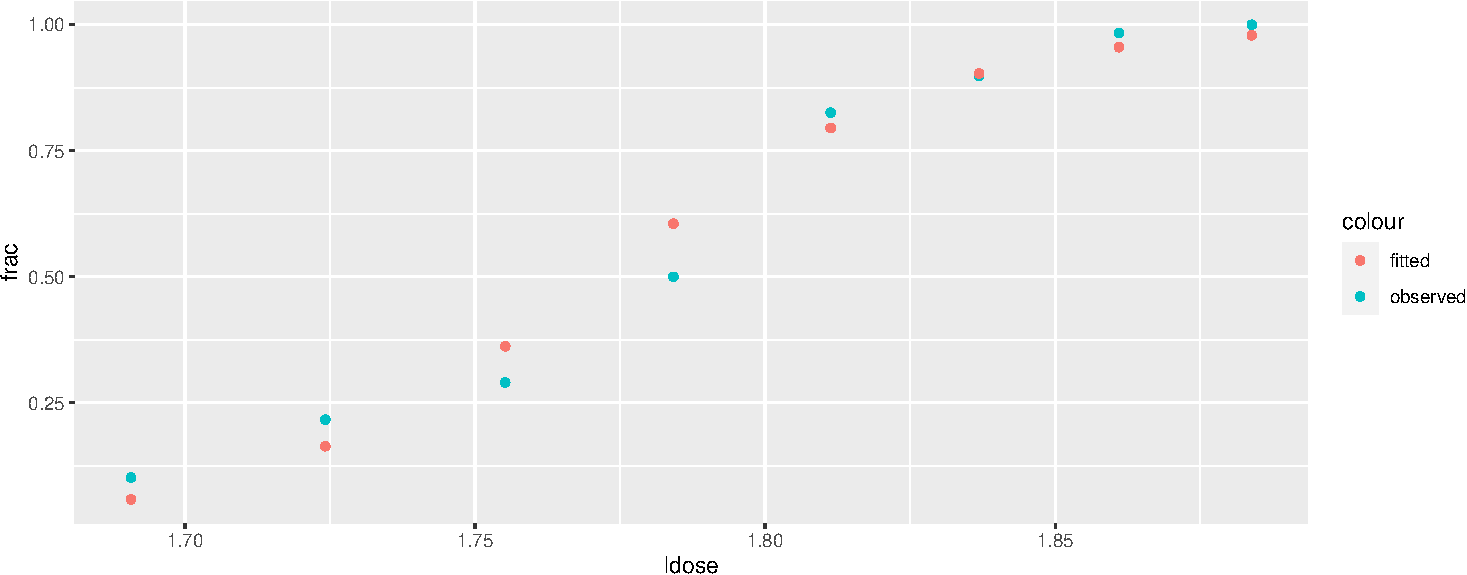
\includegraphics{Module03BinRegPresentationWeek2_files/figure-beamer/unnamed-chunk-11-1.pdf}
\end{block}
\end{frame}

\begin{frame}
\begin{block}{AIC}
\protect\hypertarget{aic}{}
It is known to us from multiple linear regression that if a model is
chosen based on a goodness of fit statistic (like the SSE or \(R^2\) in
multiple linear regression) will in general result in us choosing a to
big model (to many parameters fit). The Akaike informations criterion -
that we studied for multiple linear regression - can also be used for
binary regression: Let \(p\) be the number of regression parameters in
our model. \[\text{AIC} =-2 \cdot l(\hat{\boldsymbol{\beta}})+2p\] A
scaled version of AIC, standardizing for sample size, is sometimes
preferred.

To use AIC for model selection you use the model with the
\emph{smallest} AIC.

We may also use the BIC, where \(2p\) is replaced by \(\log(G)\cdot p\)
or \(\log(n)\cdot p\).
\end{block}
\end{frame}

\begin{frame}[fragile]
\footnotesize

\begin{Shaded}
\begin{Highlighting}[]
\FunctionTok{library}\NormalTok{(faraway)}
\NormalTok{fit1}\OtherTok{=}\FunctionTok{glm}\NormalTok{(}\FunctionTok{cbind}\NormalTok{(disease, nondisease)}\SpecialCharTok{\textasciitilde{}}\DecValTok{1}\NormalTok{,}\AttributeTok{family=}\FunctionTok{binomial}\NormalTok{(}\AttributeTok{link=}\NormalTok{logit),}\AttributeTok{data=}\NormalTok{babyfood)}
\NormalTok{fit2}\OtherTok{=}\FunctionTok{glm}\NormalTok{(}\FunctionTok{cbind}\NormalTok{(disease, nondisease)}\SpecialCharTok{\textasciitilde{}}\NormalTok{sex,}\AttributeTok{family=}\FunctionTok{binomial}\NormalTok{(}\AttributeTok{link=}\NormalTok{logit),}\AttributeTok{data=}\NormalTok{babyfood)}
\NormalTok{fit3}\OtherTok{=}\FunctionTok{glm}\NormalTok{(}\FunctionTok{cbind}\NormalTok{(disease, nondisease)}\SpecialCharTok{\textasciitilde{}}\NormalTok{food,}\AttributeTok{family=}\FunctionTok{binomial}\NormalTok{(}\AttributeTok{link=}\NormalTok{logit),}\AttributeTok{data=}\NormalTok{babyfood)}
\NormalTok{fit4}\OtherTok{=}\FunctionTok{glm}\NormalTok{(}\FunctionTok{cbind}\NormalTok{(disease, nondisease)}\SpecialCharTok{\textasciitilde{}}\NormalTok{food}\SpecialCharTok{+}\NormalTok{sex,}\AttributeTok{family=}\FunctionTok{binomial}\NormalTok{(}\AttributeTok{link=}\NormalTok{logit),}\AttributeTok{data=}\NormalTok{babyfood)}
\NormalTok{fit5}\OtherTok{=}\FunctionTok{glm}\NormalTok{(}\FunctionTok{cbind}\NormalTok{(disease, nondisease)}\SpecialCharTok{\textasciitilde{}}\NormalTok{food}\SpecialCharTok{*}\NormalTok{sex,}\AttributeTok{family=}\FunctionTok{binomial}\NormalTok{(}\AttributeTok{link=}\NormalTok{logit),}\AttributeTok{data=}\NormalTok{babyfood)}
\FunctionTok{AIC}\NormalTok{(fit1,fit2,fit3,fit4,fit5)}
\end{Highlighting}
\end{Shaded}

\begin{verbatim}
##      df      AIC
## fit1  1 59.89324
## fit2  2 56.41710
## fit3  3 43.21693
## fit4  4 40.23987
## fit5  6 43.51795
\end{verbatim}

\normalsize

\textbf{Q}: Which of these 5 models would you prefer?
\end{frame}

\begin{frame}{Overdispersion and estimating overdispersion parameter}
\protect\hypertarget{overdispersion-and-estimating-overdispersion-parameter}{}
When we have grouped data: \(Y_j \sim \text{Bin} (n_j, \pi_j)\) and
Var\((Y_j) = n_j\pi_j(1-\pi_j)\).

It is possible to estimate the variance (within a group) by
\(n_j\bar{y_j}(1-\bar{y_j})\) where \(\bar{y_j} = y_j/n_j\) (this is an
estimate of \(\pi_j\) for group \(j\)). We call this the \emph{empirical
variance}.

In a logistic regresson we estimate
\(\hat{\pi}_j = h({\bf x}_j^T\hat{\boldsymbol{\beta}})\) (\(h(\cdot)\)
is the inverse link function) which is

\[\hat{\pi_j} = \frac{\exp(x_j^T \hat{\boldsymbol{\beta}})}{1+\exp(x_j^T \hat{\boldsymbol{\beta}})} \]

for a logistic regression. This would give the \emph{estimated binomial
variance} for \(Y_j\) as \(n_j\hat{\pi_j}(1-\hat{\pi_j})\).
\end{frame}

\begin{frame}
Some times the empirical variance is much larger than the estimated
binomial variance of the model. This is called \emph{overdispersion} and
may occur when the individual responses within the groups are
correlated, or when the model could be improved upon (missing/unobserved
covariates?).

Positively correlated binary variables will give a variance of the sum
that is larger than for uncorrelated variables, e.g.

\[\text{Var}(\sum_{k=1}^K Y_k) = \sum_{k=1}^K\text{Var}(Y_k) + 2\sum_{k<l} \text{Cov}(Y_k, Y_l).\]
\end{frame}

\begin{frame}
This can be handeled by including an \emph{overdispersion parameter},
named \(\phi\), in the variance formula:

\[ \text{Var}(Y_j) = \phi n_j \pi_j (1-\pi_j)\]
\end{frame}

\begin{frame}
The overdispersion parameter can be estimated as the average Pearson
statistic or average deviance

\[\hat{\phi}_D = \frac{1}{G-p} D\]

where \(D\) is the deviance. Note that similarity to
\(\hat{\sigma^2} = 1/(n-p)\cdot\text{SSE}\) in the MLR. The
Cov\((\hat{\boldsymbol{\beta}})\) can then be changed to
\(\hat{\phi}F^{-1}(\hat{\boldsymbol{\beta}})\).

Remark: We are now moving from likelihood to quasi-likelihood theory,
where only E\((Y_j)\) and Var\((Y_j)\) - and not the distribution of
\(Y_j\) - are used in the estimation.

In Modules 7 and 8 we will look at using multilevel models to handle
correlated observations.
\end{frame}

\begin{frame}[fragile]
\begin{Shaded}
\begin{Highlighting}[]
\FunctionTok{library}\NormalTok{(investr)}
\NormalTok{estpi}\OtherTok{=}\NormalTok{investr}\SpecialCharTok{::}\NormalTok{beetle}\SpecialCharTok{$}\NormalTok{y}\SpecialCharTok{/}\NormalTok{investr}\SpecialCharTok{::}\NormalTok{beetle}\SpecialCharTok{$}\NormalTok{n}
\NormalTok{empvars}\OtherTok{=}\NormalTok{investr}\SpecialCharTok{::}\NormalTok{beetle}\SpecialCharTok{$}\NormalTok{n}\SpecialCharTok{*}\NormalTok{estpi}\SpecialCharTok{*}\NormalTok{(}\DecValTok{1}\SpecialCharTok{{-}}\NormalTok{estpi)}
\NormalTok{fit}\OtherTok{=}\FunctionTok{glm}\NormalTok{(}\FunctionTok{cbind}\NormalTok{(y, n}\SpecialCharTok{{-}}\NormalTok{y) }\SpecialCharTok{\textasciitilde{}}\NormalTok{ ldose, }\AttributeTok{family =} \StringTok{"binomial"}\NormalTok{, }\AttributeTok{data =}\NormalTok{ investr}\SpecialCharTok{::}\NormalTok{beetle)}
\NormalTok{modelestvar}\OtherTok{=}\NormalTok{investr}\SpecialCharTok{::}\NormalTok{beetle}\SpecialCharTok{$}\NormalTok{n}\SpecialCharTok{*}\NormalTok{fit}\SpecialCharTok{$}\NormalTok{fitted.values}\SpecialCharTok{*}\NormalTok{(}\DecValTok{1}\SpecialCharTok{{-}}\NormalTok{fit}\SpecialCharTok{$}\NormalTok{fitted.values)}
\FunctionTok{cbind}\NormalTok{(empvars,modelestvar)}
\end{Highlighting}
\end{Shaded}

\begin{verbatim}
##     empvars modelestvar
## 1  5.389831    3.254850
## 2 10.183333    8.227364
## 3 12.774194   14.321308
## 4 14.000000   13.378891
## 5  9.079365   10.261038
## 6  5.389831    5.156652
## 7  0.983871    2.653383
## 8  0.000000    1.230704
\end{verbatim}

\begin{Shaded}
\begin{Highlighting}[]
\NormalTok{est.dispersion}\OtherTok{=}\NormalTok{fit}\SpecialCharTok{$}\NormalTok{deviance}\SpecialCharTok{/}\NormalTok{fit}\SpecialCharTok{$}\NormalTok{df.residual }
\NormalTok{est.dispersion}
\end{Highlighting}
\end{Shaded}

\begin{verbatim}
## [1] 1.872039
\end{verbatim}

\begin{Shaded}
\begin{Highlighting}[]
\FunctionTok{summary}\NormalTok{(fit,}\AttributeTok{dispersion=}\NormalTok{est.dispersion,}\AttributeTok{correlation=}\ConstantTok{TRUE}\NormalTok{)}
\end{Highlighting}
\end{Shaded}

\begin{verbatim}
## 
## Call:
## glm(formula = cbind(y, n - y) ~ ldose, family = "binomial", data = investr::beetle)
## 
## Coefficients:
##             Estimate Std. Error z value Pr(>|z|)    
## (Intercept)  -60.717      7.088  -8.566   <2e-16 ***
## ldose         34.270      3.984   8.601   <2e-16 ***
## ---
## Signif. codes:  0 '***' 0.001 '**' 0.01 '*' 0.05 '.' 0.1 ' ' 1
## 
## (Dispersion parameter for binomial family taken to be 1.872039)
## 
##     Null deviance: 284.202  on 7  degrees of freedom
## Residual deviance:  11.232  on 6  degrees of freedom
## AIC: 41.43
## 
## Number of Fisher Scoring iterations: 4
## 
## Correlation of Coefficients:
##       (Intercept)
## ldose -1.00
\end{verbatim}

\begin{Shaded}
\begin{Highlighting}[]
\NormalTok{fitquasi}\OtherTok{=}\FunctionTok{glm}\NormalTok{(}\FunctionTok{cbind}\NormalTok{(y, n}\SpecialCharTok{{-}}\NormalTok{y) }\SpecialCharTok{\textasciitilde{}}\NormalTok{ ldose, }\AttributeTok{family =} \StringTok{"quasibinomial"}\NormalTok{, }\AttributeTok{data =}\NormalTok{ investr}\SpecialCharTok{::}\NormalTok{beetle)}
\CommentTok{\# preferred method of estimation is to use quasilikelihood}
\FunctionTok{summary}\NormalTok{(fitquasi)}\SpecialCharTok{$}\NormalTok{dispersion}
\end{Highlighting}
\end{Shaded}

\begin{verbatim}
## [1] 1.671141
\end{verbatim}
\end{frame}

\begin{frame}{References for further reading}
\protect\hypertarget{references-for-further-reading}{}
\begin{itemize}
\tightlist
\item
  A. Agresti (2015): ``Foundations of Linear and Generalized Linear
  Models.'' Wiley.
\item
  A. J. Dobson and A. G. Barnett (2008): ``An Introduction to
  Generalized Linear Models'', Third edition.
\item
  J. Faraway (2015): ``Extending the Linear Model with R'', Second
  Edition. \url{http://www.maths.bath.ac.uk/~jjf23/ELM/}
\item
  P. McCullagh and J. A. Nelder (1989): ``Generalized Linear Models''.
  Second edition.
\end{itemize}
\end{frame}

\begin{frame}
If we have time
\end{frame}

\begin{frame}
\begin{block}{Look back at MLR - what is \(s(\boldsymbol{\beta})\) and
\(F(\boldsymbol{\beta})\) then?}
\protect\hypertarget{look-back-at-mlr---what-is-sboldsymbolbeta-and-fboldsymbolbeta-then}{}
\begin{enumerate}
\item
  \(Y_i \sim \text{N}(\mu_i, \sigma^2)\)
\item
  \(\eta_j = x_i^T\boldsymbol{\beta}\)
\item
  \(\mu_i = \eta_i\) (identity response function and link function)
\end{enumerate}

Likelihood:

\[L(\boldsymbol{\beta}) = \left(\frac{1}{2\pi}\right)^{n/2}\left(\frac{1}{\sigma^2}\right)^{n/2} \exp\left(-\frac{1}{2\sigma^2}(y-{\bf X}\boldsymbol{\beta})^T(y-{\bf X}\boldsymbol{\beta})\right)\]

Loglikelihood:
\[l(\boldsymbol{\beta}) = \ln L(\boldsymbol{\beta}) = -\frac{n}{2} \ln (2\pi) - \frac{n}{2} \ln (\sigma^2) - \frac{1}{2\sigma^2}(y-{\bf X}\boldsymbol{\beta})^T(y-{\bf X}\boldsymbol{\beta})\]
\end{block}
\end{frame}

\begin{frame}
Since
\((y-{\bf X}\boldsymbol{\beta})^T(y-{\bf X}\boldsymbol{\beta}) = Y^TY - 2Y^T{\bf X}\boldsymbol{\beta} + \boldsymbol{\beta}^T{\bf X}^T{\bf X}\boldsymbol{\beta}\),
then

\[s(\boldsymbol{\beta}) = \frac{\partial l(\boldsymbol{\beta})}{\partial \boldsymbol{\beta}} = -\frac{1}{2\sigma^2}(2{\bf X}^T{\bf X}\boldsymbol{\beta}-2{\bf X}^TY) = \frac{1}{\sigma^2}({\bf X}^TY - {\bf X}^T{\bf X}\boldsymbol{\beta})\]

and \(s(\hat{\boldsymbol{\beta}}) = 0\) gives
\({\bf X}^TY - {\bf X}^T{\bf X}\boldsymbol{\beta} = 0\) which can be
solved on closed form giving
\(\hat{\boldsymbol{\beta}} = ({\bf X}^T{\bf X})^{-1}{\bf X}^TY\). So, no
need for iterative methods.
\end{frame}

\begin{frame}
Finally, observed Fisher information matrix.

\[H(\boldsymbol{\beta}) = \frac{\partial s(\boldsymbol{\beta})}{\partial \boldsymbol{\beta}^T} = -\frac{\partial}{\partial \boldsymbol{\beta}_T}(\frac{1}{\sigma^2}{\bf X}^TY - \frac{1}{\sigma^2}{\bf X}^T{\bf X}\boldsymbol{\beta}) = \frac{1}{\sigma^2}{\bf X}^T{\bf X}\]

which is independent on \(\boldsymbol{\beta}\), and also we see that
\(F(\boldsymbol{\beta})=\text{E}(H(\boldsymbol{\beta}))=H(\boldsymbol{\beta})\)
since no random variables are present. The identity link is also the
canonical link. Finally, the (asymptotic) covariance of the ML estimate
is \(F^{-1}(\hat{\boldsymbol{\beta}})=({\bf X}^T{\bf X})^{-1}\sigma^2\)
which we know as \(\text{Cov}(\hat{\boldsymbol{\beta}})\).
\end{frame}

\begin{frame}{Exponential family - and canonical link}
\protect\hypertarget{exponential-family---and-canonical-link}{}
In Module 1 we introduced distributions of the \(Y_i\), that could be
written in the form of a \emph{univariate exponential family}
\[ f(y_i\mid \theta_i)=\exp \left( \frac{y_i \theta_i-b(\theta_i)}{\phi}\cdot w_i + c(y_i, \phi, w_i) \right) \]
where

\begin{itemize}
\item
  \(\theta_i\) is called the canonical parameter and is a parameter of
  interest
\item
  \(\phi\) is called a nuisance parameter (and is not of interest to
  us=therefore a nuisance (plage))
\item
  \(w_i\) is a weight function, in most cases \(w_i=1\)
\item
  \(b\) and \(c\) are known functions.
\end{itemize}

It can be shown that \(\text{E}(Y_i)=b'(\theta_i)\) and
\(\text{Var}(Y_i)=b''(\theta_i)\cdot \frac{\phi}{w_i}\).
\end{frame}

\begin{frame}
In Module 1 we found that the binomial distribution
\(Y_i\sim \text{bin}(1,\pi_i)\) is an exponential family (derivation
from Module 1:
\url{https://www.math.ntnu.no/emner/TMA4315/2017h/Module1ExponentialFamily.pdf})

and that

\begin{itemize}
\tightlist
\item
  \(\theta_i=\ln( \frac{\pi_i}{1-\pi_i})\) is the canonical parameter
\item
  \(\phi=1\), no nuisance
\item
  \(w_i=1\)
\item
  \(b(\theta_i)=\ln(1+\exp(\theta_i))\)
\end{itemize}
\end{frame}

\begin{frame}
Recall that in a GLM we choose a link function \(g\), linking the linear
predictor and the mean: \(\eta_i=g(\mu_i)\). For the logit model we had
that \(\eta_i=\ln(\frac{\pi_i}{1-\pi_i})\).

Now (new to us) - every exponential family has a unique \emph{canonical
link function} such that \[\theta_i=\eta_i\] Since \(\eta_i=g(\mu_i)\)
this means to us that we need \[ g(\mu_i)=\theta_i\] to have a canonical
link.

\textbf{Q:} Is the logit link the canonical link for the binary model?

\textbf{A}:

Yes, since \(\theta_i=\ln( \frac{\pi_i}{1-\pi_i})=g(\pi_i)\) then the
logit link is the canonical link for the binary regression.
\end{frame}

\begin{frame}
\#\#Properties of a GLM with canonical link

\begin{enumerate}
\item
  The log-likelihod is always concave so that the ML estimated is always
  unique (given that it exists).
\item
  The observed Fisher information matrix \(H(\boldsymbol{\beta})\)
  \emph{equals} the expected Fisher information matrix
  \(F(\boldsymbol{\beta})\). That is,
  \[-\frac{\partial^2 l}{\partial \boldsymbol{\beta} \boldsymbol{\beta}^T}=\text{E}(-\frac{\partial^2 l}{\partial \boldsymbol{\beta} \boldsymbol{\beta}^T})\]
\end{enumerate}

Proving this is beyond the scope of this course.
\end{frame}

\begin{frame}{Parameter estimation - in practise}
\protect\hypertarget{parameter-estimation---in-practise}{}
To find the ML estimate \(\hat{\boldsymbol{\beta}}\) we need to solve
\[s(\hat{\boldsymbol{\beta}})=0\] We have that the score function for
the logit model is:

\[
s(\boldsymbol{\beta})=\sum_{j=1}^G {\bf x}_j (y_j-n_j\pi_j)
\]
\end{frame}

\begin{frame}
\end{frame}

\end{document}
